\section{Punto 1}
\begin{enumerate}[a)]
  \item \textit{Cómo se comportaría el algoritmo de Ordenamiento por Conteo si en el arreglo original se permiten elementos repetidos?}

  En la figura \ref{fig:Traza ordenamiento por conteo} se plantea una traza de ejemplo de como funciona el algoritmo de ordenamiento por conteo con elementos repetidos (en su descripción ademas se encuentra una referencia al repositorio donde se puede ver la imagen mas grande en caso de ser necesario)

  \begin{figure}
    \centering
    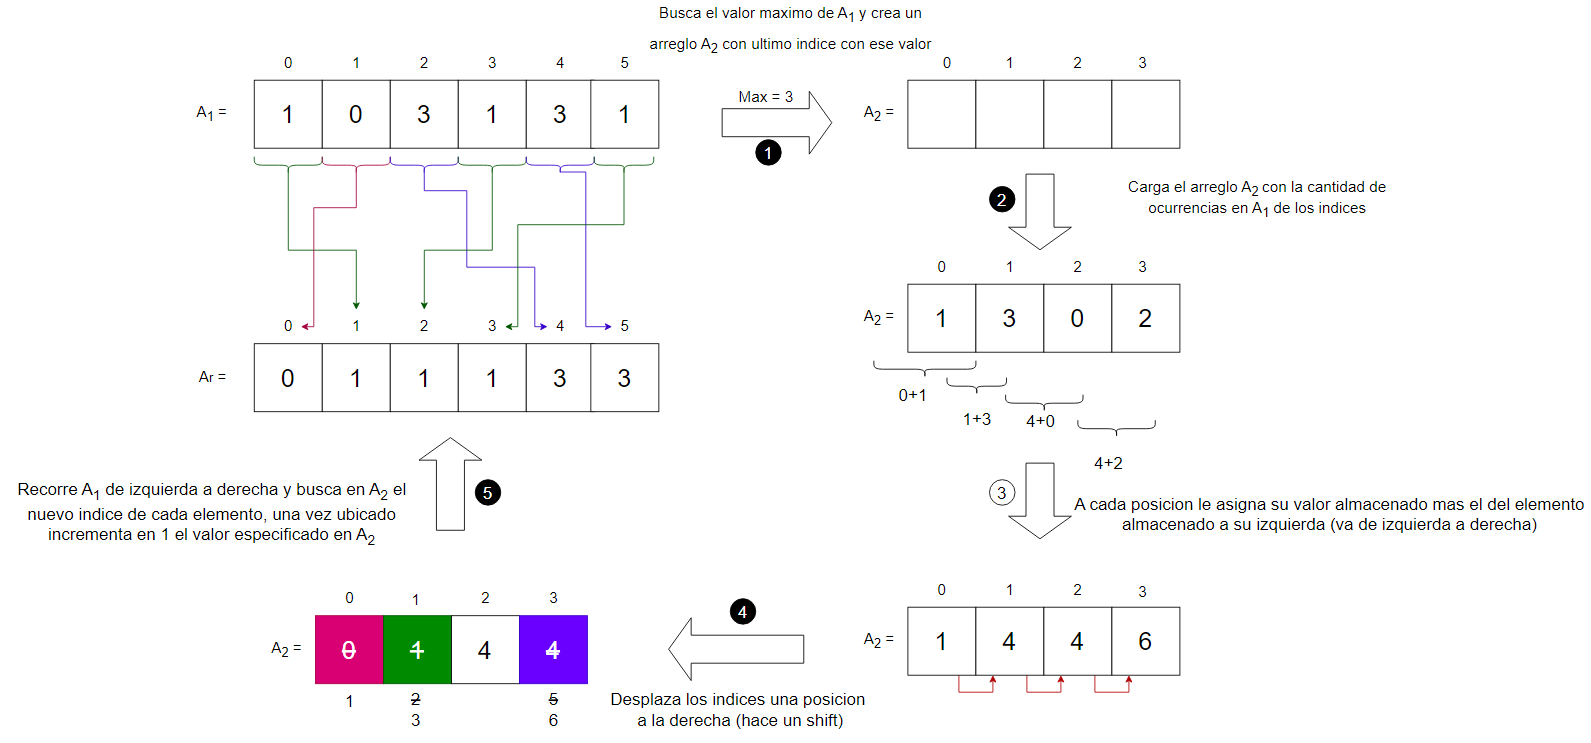
\includegraphics[width=\textwidth, scale=1]{Images/Punto1/Traza ordenamiento por conteo.png}
    \caption{Traza de algoritmo de ordenamiento por conteo \textbf{(imagen en alta resolución en \cite{trazaConteo})}}
    \label{fig:Traza ordenamiento por conteo}
  \end{figure}




  \item \textit{Modificar el algoritmo de Ordenamiento por Conteo para poder ordenar un arreglo de caracteres,
  de tal manera, que sean indistintas las letras mayúsculas y minúsculas, es decir que siempre se cumpla
  que:}\\
  $a<b$,\\
  $a<B$,\\
  $A<b$,\\
  $A<B$,\\
  \textit{En el arreglo resultante debe figurar cada letra en el mismo modo que en el arreglo original.}\\

  Para la implementación los únicos cambios respecto a un algoritmo planteado para números enteros serán la utilización el método \path{Character.compare()} para comparar caracteres y el método \path{Character.toLowerCase()} para convertir caracteres a minúsculas y asi realizar todas las comparaciones logrando la in-distinción entre letras mayúsculas y minúsculas pedida

  \begin{lstlisting}[style=java,caption= Metodo ordenarPorConteoChar]
    public static char [] ordenarPorConteoChar(char [] C){
      int n = C.length;
      int [] count = new int [n];
      char [] sorted = new char[n];
      for (int i = 0; i < n; i++) {
        count[i] = 0;
      }
      for (int i = 0; i < n-1; i++) {
        for (int j = i+1; j < n; j++) {
          if(Character.compare(Character.toLowerCase(C[i]), Character.toLowerCase(C[j]))<0){
            count[j]++;
          }else{
            count[i]++;
          }
        }
      }
      for (int i = 0; i < n; i++) {
        sorted[count[i]]=C[i];
      }
      return sorted;
    }
   \end{lstlisting}

\end{enumerate}